\documentclass[tikz,border=6pt]{standalone}
\usepackage[sfdefault,lining]{FiraSans}
\usepackage{amsmath}
\usepackage{firamath-otf}
\setmathrm{Fira Sans}
\usepackage{pgfplots}
\pgfplotsset{compat=1.18}
\usetikzlibrary{arrows.meta,calc,patterns}
\definecolor{ink}{HTML}{1F2A37}\definecolor{grey}{HTML}{6B7280}\definecolor{sea}{HTML}{1D4E89}
\definecolor{accent}{HTML}{0F766E}
\newcommand{\wavecol}[2]{\definecolor{tmpwave}{wave}{#2}\colorlet{#1}[rgb]{tmpwave}}
\begin{document}

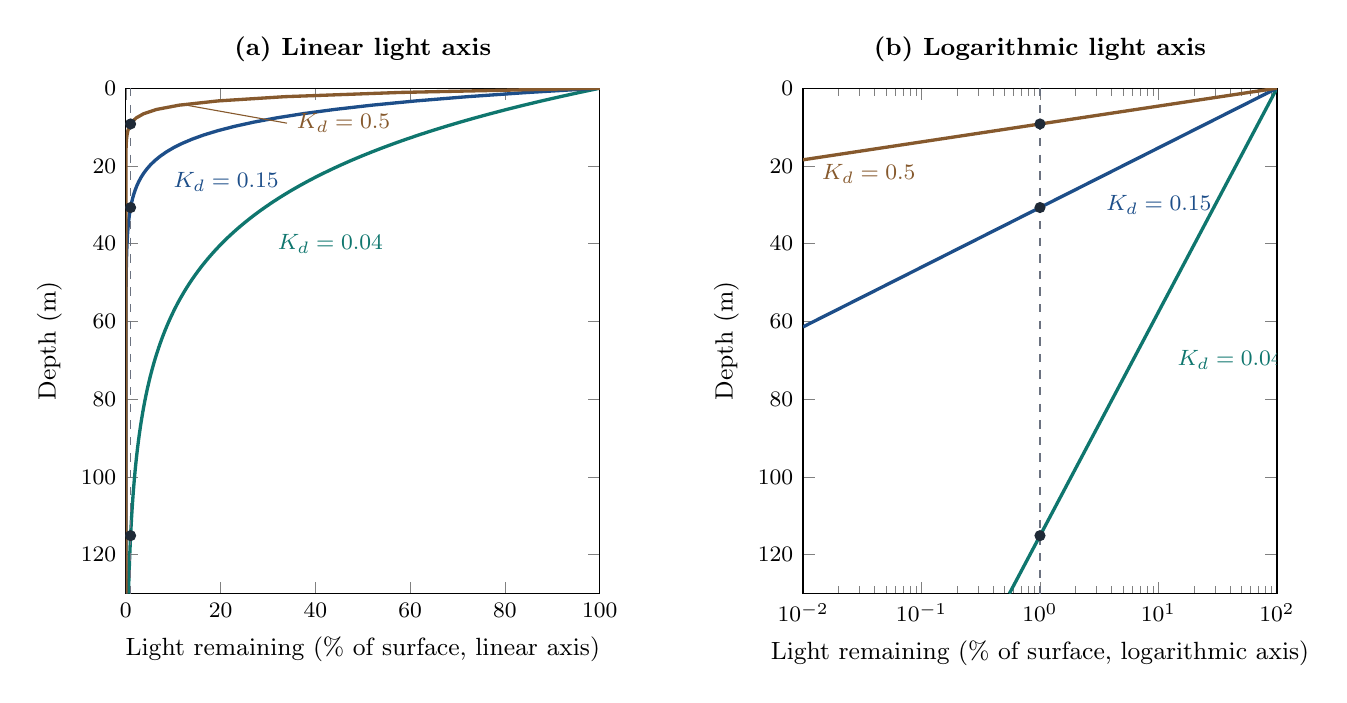
\begin{tikzpicture}
\begin{axis}[width=7.6cm,height=8cm,xmin=0,xmax=100,xlabel={Light remaining (\% of surface, linear axis)},ymin=0,ymax=130,y dir=reverse,ylabel={Depth (m)},tick label style={font=\footnotesize},label style={font=\small},title style={font=\small\bfseries},title={(a) Linear light axis}]
\addplot[very thick,accent,domain=0:130.00,samples=120] ({100*exp(-0.04*x)},{x});
\addplot[very thick,sea,domain=0:130.00,samples=120] ({100*exp(-0.15*x)},{x});
\addplot[very thick,brown!70!black,domain=0:130.00,samples=120] ({100*exp(-0.5*x)},{x});
\draw[dashed,grey] (axis cs:1,0) -- (axis cs:1,130);
\addplot[only marks,mark=*,mark size=1.8pt,ink] coordinates {(1,115.1)(1,30.7)(1,9.2)};
\node[anchor=west,font=\footnotesize\bfseries,accent] at (axis cs:30,40) {$K_d = 0.04$};
\node[anchor=west,font=\footnotesize\bfseries,sea] at (axis cs:8,24) {$K_d = 0.15$};
\draw[brown!70!black] (axis cs:12,4.2) -- (axis cs:34,9);
\node[anchor=west,font=\footnotesize\bfseries,brown!70!black] at (axis cs:34,9) {$K_d = 0.5$};
\end{axis}
\begin{scope}[xshift=8.6cm]
\begin{axis}[width=7.6cm,height=8cm,xmode=log,xmin=0.01,xmax=100,xlabel={Light remaining (\% of surface, logarithmic axis)},ymin=0,ymax=130,y dir=reverse,ylabel={Depth (m)},tick label style={font=\footnotesize},label style={font=\small},title style={font=\small\bfseries},title={(b) Logarithmic light axis}]
\addplot[very thick,accent,domain=0:130.00,samples=120] ({100*exp(-0.04*x)},{x});
\addplot[very thick,sea,domain=0:61.40,samples=120] ({100*exp(-0.15*x)},{x});
\addplot[very thick,brown!70!black,domain=0:18.42,samples=120] ({100*exp(-0.5*x)},{x});
\draw[dashed,grey] (axis cs:1,0) -- (axis cs:1,130);
\addplot[only marks,mark=*,mark size=1.8pt,ink] coordinates {(1,115.1)(1,30.7)(1,9.2)};
\node[anchor=west,font=\footnotesize\bfseries,accent] at (axis cs:12,70) {$K_d = 0.04$};
\node[anchor=west,font=\footnotesize\bfseries,sea] at (axis cs:3,30) {$K_d = 0.15$};
\node[anchor=west,font=\footnotesize\bfseries,brown!70!black] at (axis cs:0.012,22) {$K_d = 0.5$};
\end{axis}
\end{scope}
\end{tikzpicture}\end{document}